\documentclass[12pt,a4paper]{report}

% Packages
\usepackage{graphicx}
\usepackage{amsmath}
\usepackage{hyperref}
\usepackage{setspace}
\usepackage[vietnamese]{babel}
\usepackage[letterpaper,top=2cm,bottom=2cm,left=2cm,right=2cm,marginparwidth=1.75cm]{geometry}
\usepackage{listings}

% Title and Author (adjust the spacing as needed)
\title{\LARGE \textbf{PROJECT TITLE}}
\author{}
\date{\large On: \today}

% Begin Document
\begin{document}

% Title Page
\makeatletter
\begin{titlepage}
    \centering
    \vspace*{1cm}
       { 
\includegraphics[width=4cm]{UIT.jpg}}\\[0.5cm]
    {{\textbf Trường Đại học Công nghệ Thông tin\\
    Đại học Quốc gia Thành phố Hồ Chí Minh}}\\[5cm]
    {\Huge \textbf{Các ý tưởng của \\các thuật toán sắp xếp}}\\[2cm]
    
    

    
    \textbf{Cấu trúc dữ liệu và giải thuật - IT003.P21.CTTN}{}\\[1cm]
    
    \textbf{Tác giả:}{ Võ Quang Vũ }\\[1cm]
    \date{\large \today}
    {\@date\\}
\end{titlepage}
\makeatother

% Table of Contents
{\large \tableofcontents}


\pagebreak

% Chapters
\chapter{ Giới thiệu}



{\large \hspace{1cm} Trong lập trình và cả trong đời sống, các thuật toán sắp xếp luôn là một trong những đối tượng nghiên cứu quan trọng. Có rất nhiều thuật toán sắp xếp khác nhau, mỗi thuật toán có một cách hoạt động riêng, một cách sắp xếp riêng. Theo thời gian và nhu cầu sử dụng, các thuật toán sắp xếp cũng được cải tiến, nâng cấp để phù hợp với nhu cầu sử dụng. Trong bài viết này, chúng ta sẽ cùng tìm hiểu về các ý tưởng của các thuật toán sắp xếp mới dựa vào các thuật toán cũ. Các thuật toán sắp xếp được chia theo 5 thao tác trên mảng bao gồm Interchange, Insertion, Selection, Merge và được liệt kê trong bảng sau :}

\vspace*{1cm}
{ 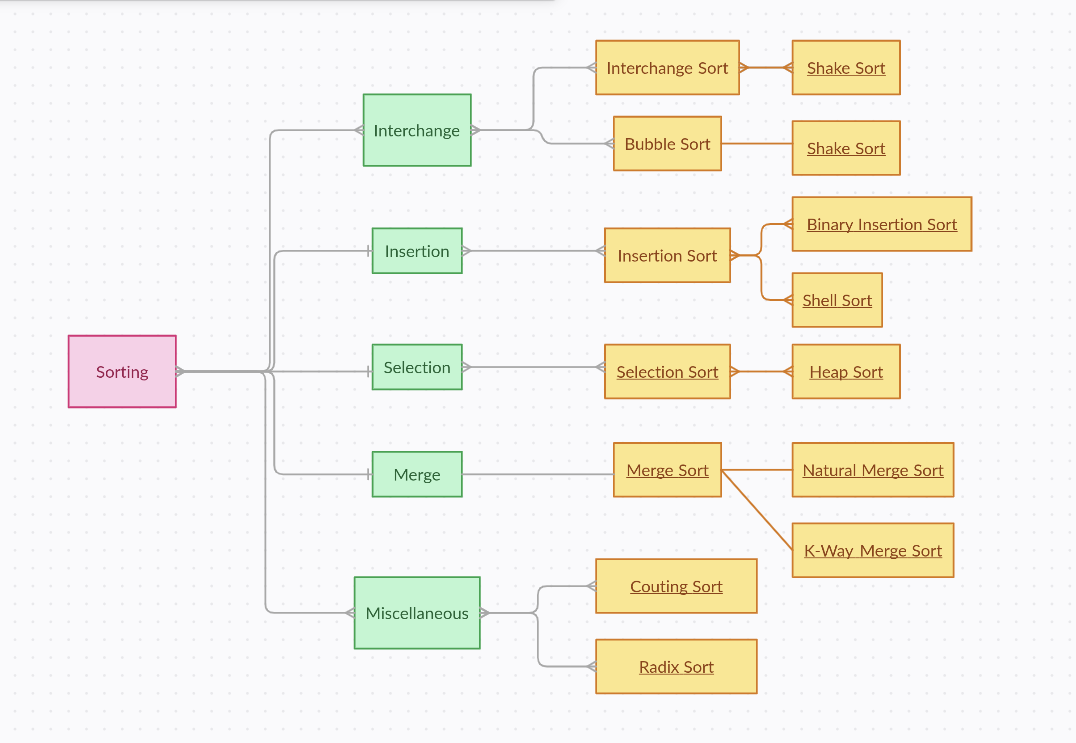
\includegraphics[width=16cm]{sort.png}}\\[0.5cm]

\large 

\chapter{ Interchange - Hoán đổi các phần tử  trong mảng}

\section{ Interchange Sort - Sắp xếp hoán đổi}
 
\subsection{ Định nghĩa}

{\large \hspace{1cm} Interchange Sort là một thuật toán sắp xếp theo nguyên lý so sánh và hoán đổi, tương tự như Bubble Sort nhưng thay vì chỉ so sánh các cặp liền kề, nó kiểm tra tất cả các cặp phần tử trong mảng. Thuật toán sẽ duyệt qua tất cả các cặp phần tử và hoán đổi chúng nếu cần, lặp lại cho đến khi toàn bộ mảng được sắp xếp.}

\subsection{ Mã giả - Mô hình thuật toán}

\begin{lstlisting}
for i = 0 to n-1 do
    for j = i+1 to n do
        if a[i] > a[j] then
            swap(a[i], a[j])
        end if
    end for
end for
\end{lstlisting}

\subsection{ Đánh giá thuật toán}

{Thời gian thực thi:

\hspace{0.5cm} Thời gian tốt nhất: O(n²) (dù mảng đã sắp xếp, thuật toán vẫn sẽ so sánh tất cả các cặp phần tử).\\

\hspace{0.5cm} Thời gian trung bình: O(n²) (do thuật toán phải kiểm tra tất cả các cặp phần tử trong mảng).\\

\hspace{0.5cm} Thời gian xấu nhất: O(n²) (trong trường hợp mảng ngược hoàn toàn).\\}

{Không gian bộ nhớ: Không gian bộ nhớ: O(1), vì thuật toán này chỉ sử dụng một số lượng bộ nhớ cố định để hoán đổi các phần tử mà không cần bộ nhớ phụ trợ lớn.}

\section{ Quick Sort - Bản nâng cấp của Interchange Sort}
 
\subsection{ Định nghĩa}

{\large \hspace{1cm} Để cải tiến thuật toán Interchange Sort, Quick Sort đã được áp dụng
kĩ thuật chia để trị để cải tiến nhưng vẫn giữ được chính bản chất là
hoán đổi vị trí. Thuật toán chia mảng thành các phần nhỏ hơn, sắp xếp các phần nhỏ hơn đó, sau đó kết hợp chúng lại với nhau để tạo ra một mảng đã sắp xếp. Quick Sort là một trong những thuật toán sắp xếp nhanh nhất hiện nay.}

\subsection {Ý tưởng mới}

Các bước Quick Sort:

Chọn pivot: Chọn một phần tử làm pivot (có thể chọn phần tử đầu, phần tử cuối, phần tử giữa hoặc ngẫu nhiên).

Phân chia mảng: Sắp xếp mảng sao cho tất cả phần tử nhỏ hơn pivot nằm ở bên trái, và tất cả phần tử lớn hơn pivot nằm ở bên phải.

Đệ quy:
Đệ quy sắp xếp phần tử bên trái của pivot.
Đệ quy sắp xếp phần tử bên phải của pivot.

\subsection{ Mã giả - Mô hình thuật toán}

\begin{lstlisting}
QuickSort(l, r):
if l < r then
    i = l
    j = r
    x = a[(l+r)/2]
    while i <= j do
        while a[i] < x do
            i = i + 1
        end while
        while a[j] > x do
            j = j - 1
        end while
        if i <= j then
            swap(a[i], a[j])
            i = i + 1
            j = j - 1
        end if
    end while
    QuickSort(l, j)
    QuickSort(i, r)
end if
\end{lstlisting}

\subsection{ Đánh giá thuật toán}

{Thời gian thực thi:

\hspace{0.5cm} Thời gian tốt nhất: O(n log n) (trong trường hợp mảng đã sắp xếp).\\

\hspace{0.5cm} Thời gian trung bình: O(n log n) (do thuật toán chia mảng thành các phần nhỏ hơn, sắp xếp các phần nhỏ hơn đó, sau đó kết hợp chúng lại với nhau để tạo ra một mảng đã sắp xếp).\\

\hspace{0.5cm} Thời gian xấu nhất: O(n²) (trong trường hợp mảng ngược hoàn toàn).\\}

{Không gian bộ nhớ: O(log n), vì thuật toán này sử dụng một số lượng bộ nhớ phụ trợ để chia mảng thành các phần nhỏ hơn.}

\section{ Bubble Sort - Sắp xếp nổi bọt}
 
\subsection{ Định nghĩa}

{\large \hspace{1cm} Interchange Sort là một thuật toán sắp xếp theo nguyên lý so sánh và hoán đổi, tương tự như Bubble Sort nhưng thay vì chỉ so sánh các cặp liền kề, nó kiểm tra tất cả các cặp phần tử trong mảng. Thuật toán sẽ duyệt qua tất cả các cặp phần tử và hoán đổi chúng nếu cần, lặp lại cho đến khi toàn bộ mảng được sắp xếp.}

\subsection{ Mã giả - Mô hình thuật toán}

\begin{lstlisting}
for i = 0 to n-1 do
    for j = i+1 to n do
        if a[i] > a[j] then
            swap(a[i], a[j])
        end if
    end for
end for
\end{lstlisting}

\subsection{ Đánh giá thuật toán}

{Thời gian thực thi:

\hspace{0.5cm} Thời gian tốt nhất: O(n²) (dù mảng đã sắp xếp, thuật toán vẫn sẽ so sánh tất cả các cặp phần tử).\\

\hspace{0.5cm} Thời gian trung bình: O(n²) (do thuật toán phải kiểm tra tất cả các cặp phần tử trong mảng).\\

\hspace{0.5cm} Thời gian xấu nhất: O(n²) (trong trường hợp mảng ngược hoàn toàn).\\}

{Không gian bộ nhớ: Không gian bộ nhớ: O(1), vì thuật toán này chỉ sử dụng một số lượng bộ nhớ cố định để hoán đổi các phần tử mà không cần bộ nhớ phụ trợ lớn.}

\section{ Shake Sort - Bản nâng cấp của Bubble Sort}
 
\subsection{ Định nghĩa}

{\large \hspace{1cm} Shake Sort là một thuật toán sắp xếp nổi bọt được cải tiến bằng cách sử dụng hai con trỏ, một con trỏ đi từ trái sang phải và một con trỏ đi từ phải sang trái. Thuật toán sẽ sắp xếp mảng bằng cách so sánh và hoán đổi các cặp phần tử như Bubble Sort, nhưng thay vì chỉ so sánh các cặp liền kề, nó kiểm tra tất cả các cặp phần tử trong mảng.}

\subsection {Ý tưởng mới}

Các bước Shake Sort:

Khởi tạo: Đặt left = 0 và right = n-1 (với n là kích thước mảng).

Duyệt từ trái sang phải:

Duyệt từ left đến right, so sánh các phần tử kề nhau và hoán đổi nếu cần.
Duyệt từ phải sang trái:

Duyệt từ right về left, so sánh các phần tử kề nhau và hoán đổi nếu cần.
Lặp lại: Tiếp tục lặp lại các bước trên cho đến khi không còn hoán đổi nào xảy ra.

\subsection{ Mã giả - Mô hình thuật toán}



\begin{lstlisting}
L=1, R=n
while L < R do
    for i = L to R-1 do
        if a[i] > a[i+1] then
            swap(a[i], a[i+1])
        end if
    end for
    R = R - 1
    for i = R-1 to L do
        if a[i] > a[i+1] then
            swap(a[i], a[i+1])
        end if
    end for
    L = L + 1
end while
\end{lstlisting}

\subsection{ Đánh giá thuật toán}

{Thời gian thực thi:

\hspace{0.5cm} Thời gian tốt nhất: O(n) (trong trường hợp mảng đã sắp xếp).\\

\hspace{0.5cm} Thời gian trung bình: O(n²) (do thuật toán phải kiểm tra tất cả các cặp phần tử trong mảng).\\

\hspace{0.5cm} Thời gian xấu nhất: O(n²) (trong trường hợp mảng ngược hoàn toàn).\\}

{Không gian bộ nhớ: Không gian bộ nhớ: O(1), vì thuật toán này chỉ sử dụng một số lượng bộ nhớ cố định để hoán đổi các phần tử mà không cần bộ nhớ phụ trợ lớn.}

\chapter{ Insertion - Chèn phần tử vào mảng}

\section{ Insertion Sort - Sắp xếp chèn}
 
\subsection{ Định nghĩa}

{\large \hspace{1cm} Insertion Sort là một thuật toán sắp xếp theo nguyên lý chèn phần tử vào vị trí đúng. Thuật toán sẽ duyệt qua từng phần tử trong mảng và chèn nó vào vị trí đúng trong mảng đã sắp xếp.}

\subsection { Ý tưởng}

Các bước Insertion Sort:

Chọn phần tử tiếp theo trong danh sách.

So sánh phần tử đó với các phần tử đã sắp xếp.

Di chuyển các phần tử đã sắp xếp sang phải để tạo không gian cho phần tử mới.

Chèn phần tử vào vị trí thích hợp.

Lặp lại cho đến khi tất cả phần tử được sắp xếp.

\pagebreak

\subsection{ Mã giả - Mô hình thuật toán}

\begin{lstlisting}
for i = 1 to n-1 do
    value = a[i]
    j = i-1
    while j >= 0 and a[j] > value do
        a[j+1] = a[j]
        j = j - 1
    end while
    a[j+1] = value
end for
\end{lstlisting}

\subsection{ Đánh giá thuật toán}

{Thời gian thực thi:

\hspace{0.5cm} Thời gian tốt nhất: O(n) (trong trường hợp mảng đã sắp xếp).\\

\hspace{0.5cm} Thời gian trung bình: O(n²) (do thuật toán phải kiểm tra tất cả các phần tử trong mảng).\\

\hspace{0.5cm} Thời gian xấu nhất: O(n²) (trong trường hợp mảng ngược hoàn toàn).\\}

{Không gian bộ nhớ: O(1), vì thuật toán này chỉ sử dụng một số lượng bộ nhớ cố định để chèn phần tử vào vị trí đúng.}



\section{ Binary Insertion Sort - Bản nâng cấp của Insertion Sort}
 
\subsection{ Định nghĩa}

{\large \hspace{1cm} Để cải tiến thuật toán Insertion Sort, Binary Insertion Sort đã được áp dụng kĩ thuật tìm kiếm nhị phân để tìm vị trí chèn phần tử vào mảng đã sắp xếp. Binary Insertion Sort sẽ tìm vị trí chèn phần tử bằng cách tìm kiếm nhị phân trong mảng đã sắp xếp thay vì so sánh tuần tự từ đầu mảng. Điều này giúp giảm số lần so sánh cần thiết để chèn phần tử vào mảng.}

\subsection {Ý tưởng mới}

Các bước Binary Insertion Sort:

Chọn phần tử tiếp theo trong danh sách.

Sử dụng tìm kiếm nhị phân để tìm vị trí chèn của phần tử.

Di chuyển các phần tử đã sắp xếp sang phải để tạo không gian.
Chèn phần tử vào vị trí tìm được.

Lặp lại cho đến khi tất cả phần tử được sắp xếp.

\subsection{ Mã giả - Mô hình thuật toán}

\begin{lstlisting}
for i = 1 to n-1 do
    value = a[i]
    left = 0
    right = i-1
    while left <= right do
        mid = (left + right) / 2
        if a[mid] > value then
            right = mid - 1
        else
            left = mid + 1
        end if
    end while
    for j = i-1 to left do
        a[j+1] = a[j]
    end for
    a[left] = value
end for
\end{lstlisting}

\subsection{ Đánh giá thuật toán}

{Thời gian thực thi:

\hspace{0.5cm} Thời gian tốt nhất: O(n log n) (trong trường hợp mảng đã sắp xếp).\\

\hspace{0.5cm} Thời gian trung bình: O(n²) (do thuật toán phải kiểm tra tất cả các phần tử trong mảng).\\

\hspace{0.5cm} Thời gian xấu nhất: O(n²) (trong trường hợp mảng ngược hoàn toàn).\\}

{Không gian bộ nhớ: O(1), vì thuật toán này chỉ sử dụng một số lượng bộ nhớ cố định để chèn phần tử vào vị trí đúng.}

\section{ Shell Sort - Bản nâng cấp của Insertion Sort}
 
\subsection{ Định nghĩa}

{\large \hspace{1cm} Tiếp nối với Binary Insertion Sort, Shell Sort là một thuật toán sắp xếp chèn được cải tiến bằng cách sử dụng một chuỗi các khoảng cách để chèn phần tử vào vị trí đúng. Shell Sort sẽ chia mảng thành các nhóm con và sắp xếp các nhóm con đó bằng thuật toán Insertion Sort. Sau đó, nó sẽ kết hợp các nhóm con lại và sắp xếp lại mảng bằng cách chèn phần tử vào vị trí đúng.}

\subsection {Ý tưởng mới}

Các bước Shell Sort:

Chọn một giá trị khoảng cách (gap).

Chia danh sách thành các nhóm con dựa trên khoảng cách.

Sắp xếp từng nhóm con bằng cách sử dụng insertion sort.

Giảm giá trị khoảng cách.

Lặp lại cho đến khi khoảng cách bằng 1.

Thực hiện một lần insertion sort cuối cùng.

\pagebreak

\subsection{ Mã giả - Mô hình thuật toán}

\begin{lstlisting}
QuickSort(l, r):
gap = n / 2
while gap > 0 do
    for i = gap to n-1 do
        value = a[i]
        j = i
        while j >= gap and a[j-gap] > value do
            a[j] = a[j-gap]
            j = j - gap
        end while
        a[j] = value
    end for
    gap = gap / 2
end while
\end{lstlisting}

\subsection{ Đánh giá thuật toán}

{Thời gian thực thi:

\hspace{0.5cm} Thời gian tốt nhất: O(n log n) (trong trường hợp mảng đã sắp xếp).\\

\hspace{0.5cm} Thời gian trung bình: O(n log² n) (do thuật toán chia mảng thành các nhóm con và sắp xếp từng nhóm con bằng thuật toán Insertion Sort).\\

\hspace{0.5cm} Thời gian xấu nhất: O(n log² n) (trong trường hợp mảng ngược hoàn toàn).\\}

{Không gian bộ nhớ: O(1), vì thuật toán này chỉ sử dụng một số lượng bộ nhớ cố định để chèn phần tử vào vị trí đúng.}

\chapter{ Selection - Chọn phần tử  trong mảng}

\section{ Selection Sort - Sắp xếp chọn}
 
\subsection{ Định nghĩa}

{\large \hspace{1cm} Selection Sort là một thuật toán sắp xếp theo nguyên lý chọn phần tử nhỏ nhất hoặc lớn nhất và đặt nó vào vị trí đúng. Thuật toán sẽ duyệt qua từng phần tử trong mảng và chọn phần tử nhỏ nhất hoặc lớn nhất để đặt vào vị trí đúng trong mảng đã sắp xếp. Sau đó, nó sẽ tiếp tục duyệt qua các phần tử còn lại và chọn phần tử tiếp theo để đặt vào vị trí đúng. Lặp lại cho đến khi toàn bộ mảng được sắp xếp.}

\subsection{ Ý tưởng}

Các bước Selection Sort:

Tìm phần tử nhỏ nhất hoặc lớn nhất trong danh sách.

Đổi chỗ phần tử đó với phần tử đầu tiên.

Tìm phần tử nhỏ nhất hoặc lớn nhất trong danh sách còn lại.

Đổi chỗ phần tử đó với phần tử thứ hai.

Lặp lại cho đến khi toàn bộ danh sách được sắp xếp.

\subsection{ Mã giả - Mô hình thuật toán}

\begin{lstlisting}
for i = 0 to n-1 do
    min = i
    for j = i+1 to n do
        if a[j] < a[min] then
            min = j
        end if
    end for
    swap(a[i], a[min])
end for
\end{lstlisting}

\subsection{ Đánh giá thuật toán}

{Thời gian thực thi:

\hspace{0.5cm} Thời gian tốt nhất: O(n²) (dù mảng đã sắp xếp, thuật toán vẫn phải duyệt qua tất cả các phần tử).\\

\hspace{0.5cm} Thời gian trung bình: O(n²) (do thuật toán phải duyệt qua tất cả các phần tử trong mảng).\\

\hspace{0.5cm} Thời gian xấu nhất: O(n²) (trong trường hợp mảng ngược hoàn toàn).\\}

{Không gian bộ nhớ: O(1), vì thuật toán này chỉ sử dụng một số lượng bộ nhớ cố định để hoán đổi các phần tử mà không cần bộ nhớ phụ trợ lớn.}

\section{ Heap Sort - Bản nâng cấp của Selection Sort}
 
\subsection{ Định nghĩa}

{\large \hspace{1cm} Để cải tiến thuật toán Selection Sort, Heap Sort đã được áp dụng kĩ thuật heap để chọn phần tử lớn nhất hoặc nhỏ nhất và đặt nó vào vị trí đúng. Heap Sort sẽ chuyển mảng thành một cây heap và chọn phần tử lớn nhất hoặc nhỏ nhất để đặt vào vị trí đúng. Sau đó, nó sẽ tiếp tục chuyển mảng thành cây heap và chọn phần tử tiếp theo để đặt vào vị trí đúng. Lặp lại cho đến khi toàn bộ mảng được sắp xếp.}

\subsection {Ý tưởng mới}

Các bước Quick Sort:

Xây dựng heap từ danh sách ban đầu (max-heap).

Đổi chỗ phần tử đầu (max) với phần tử cuối.

Giảm kích thước heap.

Thực hiện heapify lại từ gốc.

Lặp lại bước 2-4 cho đến khi heap chỉ còn một phần tử.

\subsection{ Mã giả - Mô hình thuật toán}

\begin{lstlisting}
for i = 1 to N
    min = heap.get_min()
    heap.remove_min()
    swap(a[i], a[min])
\end{lstlisting}

\subsection{ Đánh giá thuật toán}

{Thời gian thực thi:

\hspace{0.5cm} Thời gian tốt nhất: O(n log n) (trong trường hợp mảng đã sắp xếp).\\

\hspace{0.5cm} Thời gian trung bình: O(n log n) (do thuật toán chuyển mảng thành cây heap và chọn phần tử lớn nhất hoặc nhỏ nhất để đặt vào vị trí đúng).\\

\hspace{0.5cm} Thời gian xấu nhất: O(n log n) (trong trường hợp mảng ngược hoàn toàn).\\}

{Không gian bộ nhớ: O(1), vì thuật toán này chỉ sử dụng một số lượng bộ nhớ cố định để hoán đổi các phần tử mà không cần bộ nhớ phụ trợ lớn.}

\chapter{ Merge - Trộn các phần tử của mảng này vào mảng khác}

Ý tưởng của việc merge các phần tử của mảng là kết hợp hai mảng đã sắp xếp thành một mảng mới đã sắp xếp. Có nhiều cách để merge hai mảng đã sắp xếp, nhưng cách phổ biến nhất là sử dụng phương pháp gộp hai mảng đã sắp xếp thành một mảng mới đã sắp xếp. Bằng thuật toán hai con trỏ, ta có thể gộp hai mảng đã sắp xếp thành một mảng mới đã sắp xếp trong độ phức tạp thời gian O(n). Pseudocode: 

\begin{lstlisting}
a[n], b[m], c[n+m]
i = 0, j = 0, k = 0
while i < n and j < m do
    if a[i] < b[j] then
        c[k] = a[i]
        i = i + 1
    else
        c[k] = b[j]
        j = j + 1
    end if
    k = k + 1
end while
\end{lstlisting}



\section{ Merge Sort - Sắp xếp trộn}
 
\subsection{ Định nghĩa}

{\large \hspace{1cm} Merge Sort là một thuật toán sắp xếp theo nguyên lý chia để trị, tương tự như Quick Sort nhưng thay vì chia mảng thành các phần nhỏ hơn, nó chia mảng thành hai phần bằng nhau và sắp xếp từng phần đó. Sau đó, nó sẽ gộp hai phần đã sắp xếp thành một mảng đã sắp xếp.}

\subsection { Ý tưởng}

Sử dụng thuật toán hai con trỏ trên, ta kết hợp đệ quy để gộp hai mảng đã sắp xếp thành một mảng mới đã sắp xếp. Bằng cách chia mảng thành các phần nhỏ hơn, sắp xếp các phần nhỏ hơn đó, sau đó kết hợp chúng lại với nhau để tạo ra một mảng đã sắp xếp.

\subsection{ Mã giả - Mô hình thuật toán}

\begin{lstlisting}
Merge(l, m, r):
    n1 = m - l + 1
    n2 = r - m
    L[n1], R[n2]
    for i = 0 to n1-1 do
        L[i] = a[l+i]
    end for
    for j = 0 to n2-1 do
        R[j] = a[m+1+j]
    end for
    i = 0, j = 0, k = l
    while i < n1 and j < n2 do
        if L[i] <= R[j] then
            a[k] = L[i]
            i = i + 1
        else
            a[k] = R[j]
            j = j + 1
        end if
        k = k + 1
    end while
    while i < n1 do
        a[k] = L[i]
        i = i + 1
        k = k + 1
    end while
    while j < n2 do
        a[k] = R[j]
        j = j + 1
        k = k + 1
    end while

MergeSort (l, r):
if l < r then
    m = (l+r) / 2
    MergeSort(l, m)
    MergeSort(m+1, r)
    Merge(l, m, r)
end if
\end{lstlisting}

\subsection{ Đánh giá thuật toán}

{Thời gian thực thi:

\hspace{0.5cm} Thời gian tốt nhất: O(n log n) (trong trường hợp mảng đã sắp xếp).\\

\hspace{0.5cm} Thời gian trung bình: O(n log n) (do thuật toán chia mảng thành các phần nhỏ hơn, sắp xếp các phần nhỏ hơn đó, sau đó kết hợp chúng lại với nhau để tạo ra một mảng đã sắp xếp).\\

\hspace{0.5cm} Thời gian xấu nhất: O(n log n) (trong trường hợp mảng ngược hoàn toàn).\\}

{Không gian bộ nhớ: O(n), vì thuật toán này sử dụng một số lượng bộ nhớ phụ trợ để chia mảng thành các phần nhỏ hơn.}

\section{ Natural Merge Sort - Bản nâng cấp của Merge Sort}
 
\subsection{ Định nghĩa}

{\large \hspace{1cm} Để cải tiến thuật toán Merge Sort, Natural Merge Sort đã được áp dụng kĩ thuật tìm kiếm nhị phân để tìm các phần tử đã sắp xếp và gộp chúng lại với nhau. Natural Merge Sort sẽ tìm các phần tử đã sắp xếp trong mảng và gộp chúng lại với nhau để tạo ra một mảng mới đã sắp xếp. Điều này giúp giảm số lần so sánh cần thiết để gộp các phần tử đã sắp xếp.}

\subsection {Ý tưởng mới}

Các bước Natural Merge Sort:

Tìm các phần tử đã sắp xếp trong mảng.

Gộp các phần tử đã sắp xếp lại với nhau.

Lặp lại cho đến khi toàn bộ mảng được sắp xếp.

\subsection{ Mã giả - Mô hình thuật toán}

\begin{lstlisting}
MergeSort (l, r):
if l < r then
    if issorted(l, r) then
        return
    end if
    m = (l+r) / 2
    MergeSort(l, m)
    MergeSort(m+1, r)
    Merge(l, m, r)
end if
\end{lstlisting}

\subsection{ Đánh giá thuật toán}

{Thời gian thực thi:

\hspace{0.5cm} Thời gian tốt nhất: O(n log n) (trong trường hợp mảng đã sắp xếp).\\

\hspace{0.5cm} Thời gian trung bình: O(n log n) (do thuật toán tìm các phần tử đã sắp xếp trong mảng và gộp chúng lại với nhau để tạo ra một mảng mới đã sắp xếp).\\

\hspace{0.5cm} Thời gian xấu nhất: O(n log n) (trong trường hợp mảng ngược hoàn toàn).\\}

{Không gian bộ nhớ: O(n), vì thuật toán này sử dụng một số lượng bộ nhớ phụ trợ để tìm các phần tử đã sắp xếp trong mảng và gộp chúng lại với nhau.}

\section{ K-Way Merge Sort - Merge Sort với K mảng khác nhau}
 
\subsection{ Định nghĩa}

{\large \hspace{1cm} Để cải tiến thuật toán Merge Sort, K-Way Merge Sort đã được áp dụng kĩ thuật gộp K mảng khác nhau thành một mảng mới đã sắp xếp. K-Way Merge Sort sẽ gộp K mảng khác nhau thành một mảng mới đã sắp xếp. Điều này giúp giảm số lần so sánh cần thiết để gộp các mảng khác nhau. }

\subsection {Ý tưởng mới}

Các bước K-Way Merge Sort:

Gộp K mảng khác nhau thành một mảng mới đã sắp xếp.

Lặp lại cho đến khi toàn bộ mảng được sắp xếp.

\subsection{ Mã giả - Mô hình thuật toán}

\begin{lstlisting}
a[], b[][], id[]
KMergeSort (a[1..n], k):
    tmp = -1
    for i = 1 to n do 
        for j = 1 to k do 
            if (id[j] <= size[j]) 
            and (u==-1 or B[j][id[j] < B[u][id[u]]) then
                u = j
            end if
        end for
        a.insert(B[u][id[u]])
        id[u] = id[u] + 1
    end for
\end{lstlisting}

\subsection{ Đánh giá thuật toán}

{Thời gian thực thi:

\hspace{0.5cm} Thời gian tốt nhất: O(n log n) (trong trường hợp mảng đã sắp xếp).\\

\hspace{0.5cm} Thời gian trung bình: O(n log n) (do thuật toán gộp K mảng khác nhau thành một mảng mới đã sắp xếp).\\

\hspace{0.5cm} Thời gian xấu nhất: O(n log n) (trong trường hợp mảng ngược hoàn toàn).\\}

{Không gian bộ nhớ: O(n), vì thuật toán này sử dụng một số lượng bộ nhớ phụ trợ để gộp K mảng khác nhau thành một mảng mới đã sắp xếp.}

\chapter { Các thuật toán sắp xếp khác}

\section{ Counting Sort - Sắp xêp đếm}
 
\subsection{ Định nghĩa}

{\large \hspace{1cm} Counting Sort là một thuật toán sắp xếp theo nguyên lý đếm số lần xuất hiện của mỗi phần tử trong mảng. Thuật toán sẽ duyệt qua từng phần tử trong mảng và đếm số lần xuất hiện của mỗi phần tử. Sau đó, nó sẽ tạo một mảng mới chứa số lần xuất hiện của mỗi phần tử và sắp xếp mảng mới đó.}

\subsection{ Ý tưởng}

Giả sử ta có mảng A 

Ta tạo một mảng B với kích thước bằng với giá trị lớn nhất trong dãy A

Ta duyệt qua từng phần tử trong dãy A, tăng giá trị tại vị trí tương ứng trong mảng B lên 1

Ta duyệt qua từng phần tử trong mảng B, nếu giá trị tại vị trí đó lớn hơn 0 thì in ra giá trị đó

\subsection{ Mã giả - Mô hình thuật toán}

\begin{lstlisting}
cnt[]
a[], b[]
CountingSort (a[1..n]):
    for i = 1 to n do
        cnt[a[i]] = cnt[a[i]] + 1
    end for
    k = 1
    for i = 1 to max do
        for j = 1 to cnt[i] do
            a[k] = i
            k = k + 1
            b.insert(i)
        end for
    end for
\end{lstlisting}

\subsection{ Đánh giá thuật toán}

{Thời gian thực thi:

\hspace{0.5cm} Thời gian tốt nhất: O(n) (trong trường hợp mảng đã sắp xếp).\\

\hspace{0.5cm} Thời gian trung bình: O(n) (do thuật toán đếm số lần xuất hiện của mỗi phần tử trong mảng).\\

\hspace{0.5cm} Thời gian xấu nhất: O(n) (trong trường hợp mảng ngược hoàn toàn).\\}

{Không gian bộ nhớ: O(n), vì thuật toán này sử dụng một số lượng bộ nhớ phụ trợ để đếm số lần xuất hiện của mỗi phần tử trong mảng.}

\section{ Radix Sort - Sắp xếp cơ số}

\subsection{ Định nghĩa}

{\large \hspace{1cm} Radix Sort là một thuật toán sắp xếp theo nguyên lý sắp xếp từng chữ số của mỗi phần tử trong mảng. Thuật toán sẽ duyệt qua từng chữ số của mỗi phần tử trong mảng và sắp xếp chúng theo thứ tự từ bé đến lớn hoặc từ lớn đến bé.}

\subsection{ Ý tưởng}

Các bước Radix Sort:

Xác định số chữ số lớn nhất trong dãy.

Sắp xếp các phần tử theo chữ số (từ phải sang trái) bằng cách sử dụng counting sort.

Lặp lại cho đến khi sắp xếp xong tất cả các chữ số.

\subsection{ Mã giả - Mô hình thuật toán}

\begin{lstlisting}
Group[10][]
Groupsize[10]
RadixSort()
    max = findmax()
    for i = 0 to max do
        for j = 0 to n do
            Group[a[j] % 10].insert(a[j])
            Groupsize[a[j] % 10] = Groupsize[a[j] % 10] + 1
            a[j] = a[j] / 10
        end for
        k = 0
        for j = 0 to 9 do
            for l = 0 to Groupsize[j] do
                a[k] = Group[j][l]
                k = k + 1
            end for
        end for
    end for
\end{lstlisting}

\subsection{ Đánh giá thuật toán}

{Thời gian thực thi:

\hspace{0.5cm} Thời gian tốt nhất: O(nk) (trong trường hợp mảng đã sắp xếp).\\

\hspace{0.5cm} Thời gian trung bình: O(nk) (do thuật toán sắp xếp từng chữ số của mỗi phần tử trong mảng).\\

\hspace{0.5cm} Thời gian xấu nhất: O(nk) (trong trường hợp mảng ngược hoàn toàn).\\}

{Không gian bộ nhớ: O(n), vì thuật toán này sử dụng một số lượng bộ nhớ phụ trợ để sắp xếp từng chữ số của mỗi phần tử trong mảng.}

\end{document}